% $Header: /cvsroot/latex-beamer/latex-beamer/solutions/generic-talks/generic-ornate-15min-45min.en.tex,v 1.5 2007/01/28 20:48:23 tantau Exp $

\documentclass[letter,graphicx]{beamer}

% This file is a solution template for:

% - Giving a talk on some subject.
% - The talk is between 15min and 45min long.
% - Style is ornate.



% Copyright 2004 by Till Tantau <tantau@users.sourceforge.net>.
%
% In principle, this file can be redistributed and/or modified under
% the terms of the GNU Public License, version 2.
%
% However, this file is supposed to be a template to be modified
% for your own needs. For this reason, if you use this file as a
% template and not specifically distribute it as part of a another
% package/program, I grant the extra permission to freely copy and
% modify this file as you see fit and even to delete this copyright
% notice. 


\mode<presentation>
{
  \usetheme{Warsaw}
  % or ...

  \setbeamercovered{transparent}
  \setbeamertemplate{footling}[frame number]
  % or whatever (possibly just delete it)
}


\usepackage[english]{babel}
% or whatever

\usepackage[latin1]{inputenc}
% or whatever
\usepackage{verbatim}
\usepackage{times}
\usepackage[T1]{fontenc}
%\usepackage{mychicago}
%\renewcommand{\citeN}{\shortciteN}
% Or whatever. Note that the encoding and the font should match. If T1
% does not look nice, try deleting the line with the fontenc.

\logo{
\includegraphics[width=.1\textwidth]{./images/official_NOAA_logo.pdf}}

\title[SNP contamination identification with Bayesian methods\hspace{2em}\insertframenumber] % (optional, use only with long paper titles)
{Algorithms for Identifying Contaminated Samples Genotyped with Single Nucleotide Polymorphisms}

\subtitle{} % (optional)

\author[Elena Venable] % (optional, use only with lots of authors)
{Elena Venable}
% - Use the \inst{?} command only if the authors have different
%   affiliation.

\institute[Brown Univeristy] % (optional, but mostly needed)
{
Brown University \\ Applied Mathematics - Biology \\ Healthy Oceans \\ Southwest Fisheries Science Center, Santa Cruz, CA \\ Eric C. Anderson
}
% - Use the \inst command only if there are several affiliations.
% - Keep it simple, no one is interested in your street address.

\date[CSGM--2014] % (optional)
{
 Hollings and EPP Undergraduate Scholars Symposium \\ 29 AUGUST 2014}

\subject{Talks}
% This is only inserted into the PDF information catalog. Can be left
% out. 



% If you have a file called "university-logo-filename.xxx", where xxx
% is a graphic format that can be processed by latex or pdflatex,
% resp., then you can add a logo as follows:

% \pgfdeclareimage[height=0.5cm]{university-logo}{university-logo-filename}
% \logo{\pgfuseimage{university-logo}}

% Delete this, if you do not want the table of contents to pop up at
% the beginning of each subsection:
%\AtBeginSection[]
%{
%  \begin{frame}<beamer>{Outline}
%    \tableofcontents[currentsection,currentsubsection]
%  \end{frame}
%}
% If you wish to uncover everything in a step-wise fashion, uncomment
% the following command: 

%\beamerdefaultoverlayspecification{<+->}

%% More eric commands for inserting some small figures
%\newcommand{\smikid}{\includegraphics[width=3.7ex]{images/smiley_blue_kid.pdf}}
%\newcommand{\smired}{\includegraphics[width=2.9ex]{images/smiley_sad_red.png}}
%\newcommand{\smiblue}{\includegraphics[width=2.9ex]{images/smiley_happy_blue.png}}
%\newcommand{\thh}{^\mathrm{th}}
%\newcommand{\tc}{\textcolor}
%\def\bm#1{\mathpalette\bmstyle{#1}}
%\def\bmstyle#1#2{\mbox{\boldmath$#1#2$}}


\begin{document}

%Slide 1
\begin{frame}
  \titlepage
\end{frame}

%Slide 2
\begin{frame}{Overview}
   \begin{itemize}
	\item Introduction/Objectives
	\item Background Theory
	\item Single Population Model
	\item Mixture Model
	\item Next Steps
	\item Conclusion
   \end{itemize}
\end{frame}

%Slide 3
\begin{frame}{Introduction/Objectives}
   \begin{itemize}
	\item  Importance of stock identification for protecting endangered population of salmon along the West Coast
	\item New stock identification technology using Single Nucleotide Polymorphisms developed at the Southwest Fisheries Science Center
   \end{itemize}
\end{frame}

%Slide 4
\begin{frame}{Background Theory}
\framesubtitle{Single Nucleotide Polymorphisms (SNPs)}
Some short description and a picture to explain SNPs.
\end{frame}

%Slide 5
\begin{frame}{Background Theory}
\framesubtitle{Statistical Models}
   \begin{itemize}
   	\item Logic of identify based on heterozygousity
	\item Bayesian Approach
   \end{itemize}
\end{frame}

%Slide 6
\begin{frame}{Background Theory}
\framesubtitle{Bayesian Statistics}
Short explanation of Bayesian statistics and maybe include a few equations with prior, posterior distributions, etc. 
\end{frame}

%Slide 7
\begin{frame}{Single Population Model}
\begin{columns}[c]

\column{2.25in}
%\begin{itemize}
$\boldsymbol{\rho}$: contamination proportion \\
\vspace{3mm}
$\boldsymbol{z_i}$: contamination indicator \\
\vspace{3mm}
$\boldsymbol{y_{i,\ell}}$: genotype \\
\vspace{3mm}
$\boldsymbol{\theta_{\ell}}$: allele frequency \\
\vspace{3mm}
$\boldsymbol{\alpha}, \pmb{\beta}, \boldsymbol{\lambda}$: distribution parameters
%\end{itemize}

\column{2in}
\begin{center}
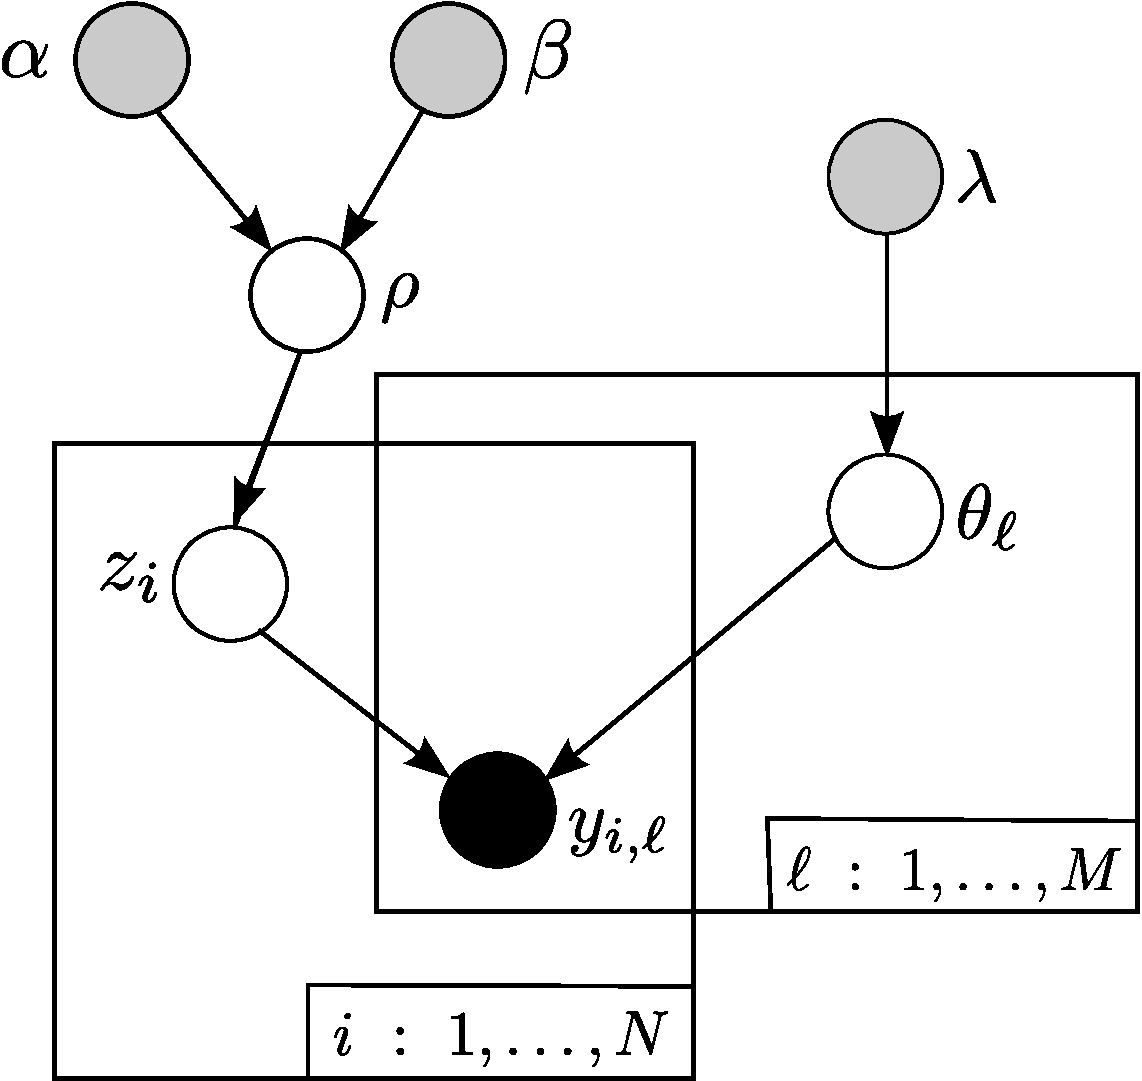
\includegraphics[width=1\textwidth]{images/DAG_1.pdf}
\end{center}
\end{columns}
\end{frame}

%Slide 8
\begin{frame}{Single Population Model}
\framesubtitle{Simulation}
\end{frame}

%Slide 9
\begin{frame}{Single Population Model}
\framesubtitle{Results}
\begin{columns}[b]

\column{2in}
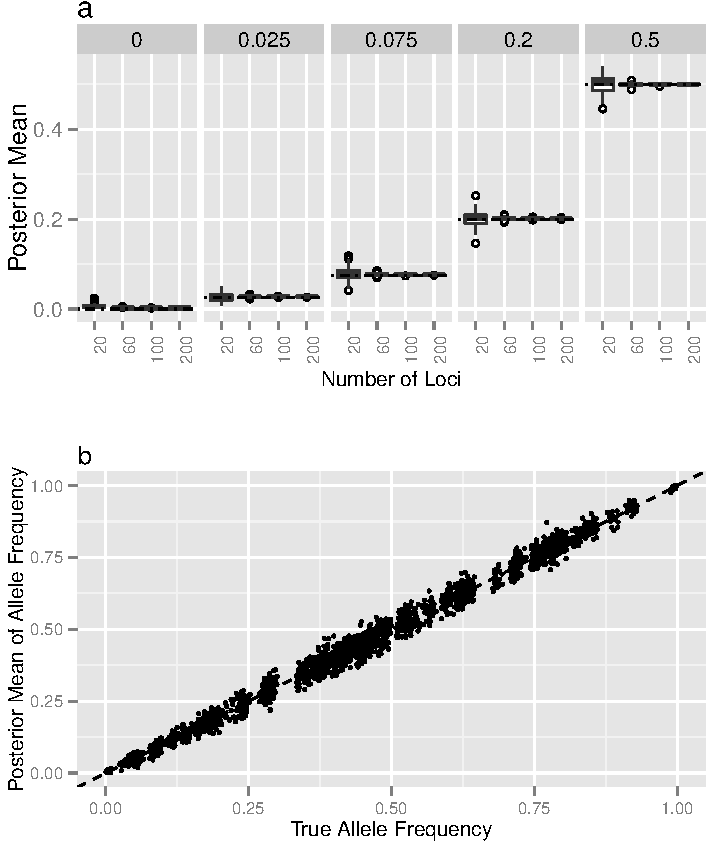
\includegraphics[width=1\textwidth]{images/rho_and_allele.pdf}

\column{2.25in}
\begin{itemize}
\item contamination proportion is estimated very well
\vspace{3mm}
\item also good estimation of allele frequencies
\end{itemize}

\begin{table}
\hrule \hrule
\begin{center}
\begin{scriptsize}
\begin{tabular}{lrrrr} 
  &  \multicolumn{4}{c}{\underline{Number of Loci, $L$}} \\
$\rho$~~~~~~~~~~  &  20                 &  60                 &  100                &  200                \\  
\hline 0          &  0.91               &  0.90               &  0.90               &  0.90               \\  
0.025              &  0.90               &  0.90               &  0.90               &  0.90               \\  
0.075              &  0.90               &  0.90               &  0.90               &  0.89               \\  
0.2                &  0.91               &  0.90               &  0.90               &  0.90               \\  
0.5                &  0.92               &  0.90               &  0.90               &  0.90               \\  
\end{tabular} 

\end{scriptsize}
\end{center}
\hrule
\end{table}

\end{columns}
\end{frame} 

%Slide 10
\begin{frame}{Single Population Model}
\framesubtitle{Results}
\begin{columns}[c]
\column{2.25in}
\begin{table}
\begin{scriptsize}
\hrule\hrule
\mbox{}\\
{\bf (a)} Contaminated samples 
\begin{center}
\begin{tabular}{lrrrr} 
  &  \multicolumn{4}{c}{\underline{Number of Loci, $L$}} \\
$\rho~~~~~~~$  &  20              &  60              &  100             &  200             \\  
\hline 0.025   &  0.612           &  0.984           &  1.000           &  1.000           \\  
0.075           &  0.765           &  0.990           &  0.999           &  1.000           \\  
0.2             &  0.870           &  0.994           &  1.000           &  1.000           \\  
0.5             &  0.944           &  0.996           &  1.000           &  1.000           \\  
\end{tabular} 
\end{center}
{\bf (b)} Non-contaminated samples 
\begin{center}
\begin{tabular}{lrrrr} 
  &  \multicolumn{4}{c}{\underline{Number of Loci, $L$}} \\
$\rho~~~~~~~$  &  20              &  60              &  100             &  200             \\  
\hline 0       &  0.0010          &  0.0000          &  0.0000          &  0.0000          \\  
0.025           &  0.0030          &  0.0003          &  0.0000          &  0.0000          \\  
0.075           &  0.0124          &  0.0010          &  0.0000          &  0.0000          \\  
0.2             &  0.0239          &  0.0016          &  0.0000          &  0.0000          \\  
0.5             &  0.0618          &  0.0028          &  0.0001          &  0.0000          \\  
\end{tabular} 
\end{center}

\hrule
\end{scriptsize}
\end{table}

\column{2.25in}
\begin{itemize}
\item true positives \textbf{(a)} and false negatives \textbf{(b)}
\vspace{3mm}
\item with large $L$, almost all contaminated samples identified, with practically zero false identifications
\vspace{3mm}
\item even with small $L$, most contaminated samples are identified with few errors
\end{itemize}
\end{columns}
\end{frame}

%Slide 11
\begin{frame}{Mixture Model}
\begin{columns}[c]

\column{2in}
%\begin{itemize}
$\boldsymbol{\pi}$: mixing proportions \\
\vspace{3mm}
$\boldsymbol{u_i}$: population indicator \\
\vspace{3mm}
$\boldsymbol{B}$: baseline data\\
\vspace{3mm}
$\boldsymbol{\xi}$: distribution parameter
%\end{itemize}

\column{2.25in}
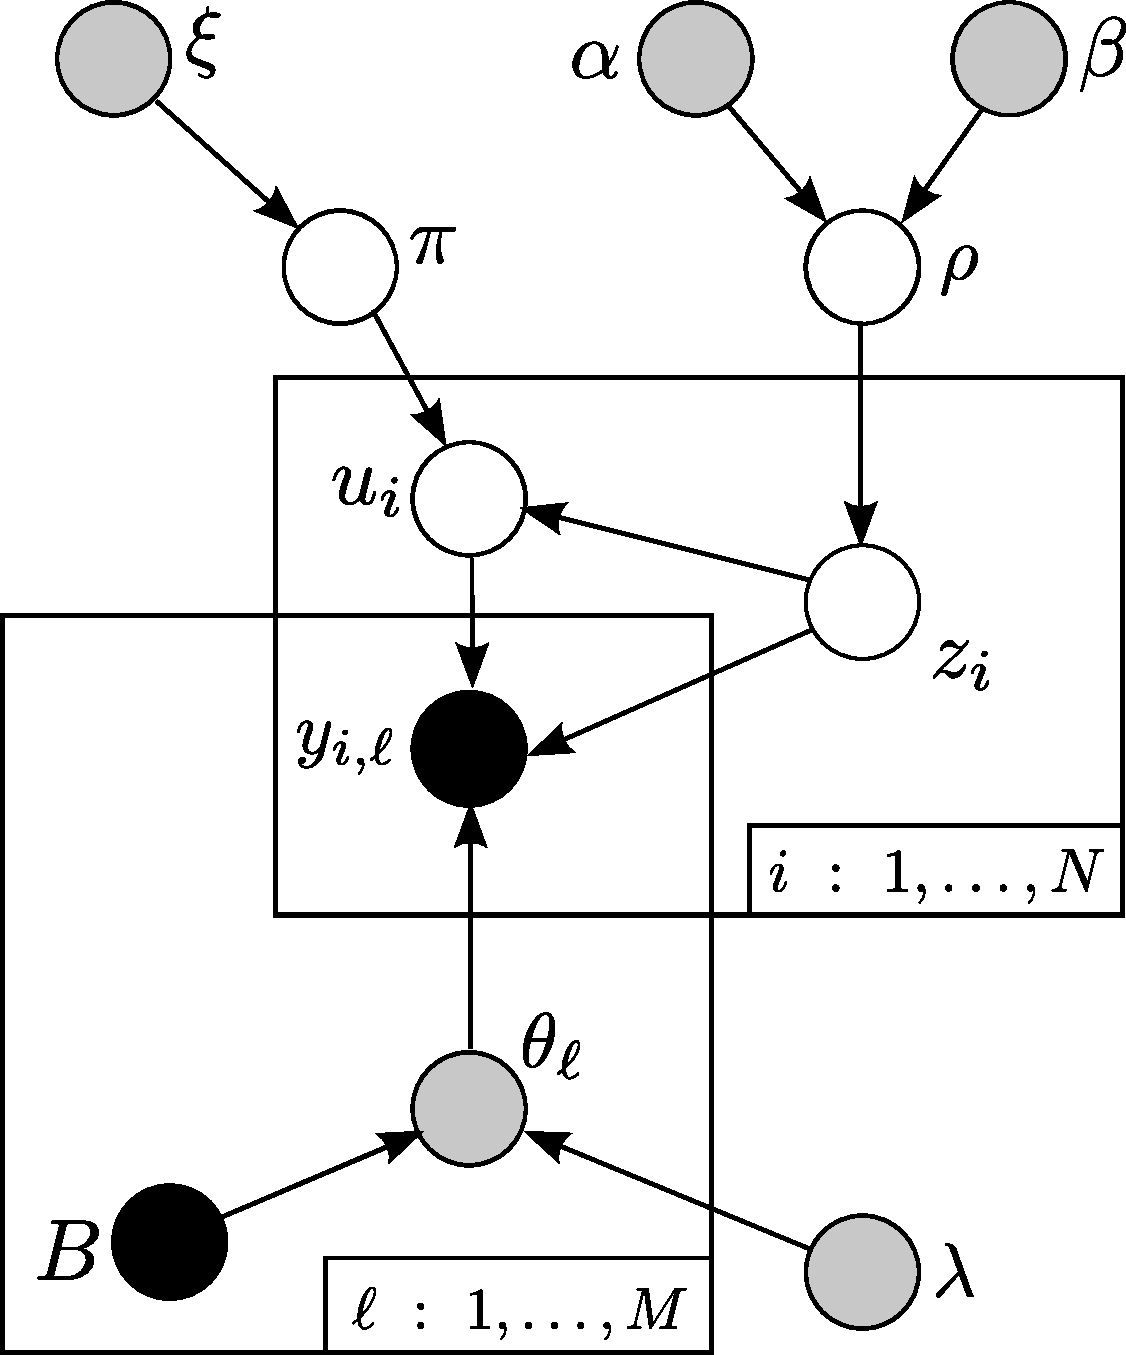
\includegraphics[width=.9\textwidth]{images/DAG_2.pdf}

\end{columns}
\end{frame}

%Slide12
\begin{frame}{Mixture Model}
\framesubtitle{Simulation}
\end{frame}

%Slide 13
\begin{frame}{Mixture Model}
\framesubtitle{Results}
\end{frame} 
 
%Slide 14
\begin{frame}{Next Steps}
\end{frame}

%Slide 15
\begin{frame}{Conclusion}
\end{frame}

%Slide 16
\begin{frame}{Mathematics}
\end{frame} 

\end{document}